\newpage
\chapter{Quick start} \SecLabel{QuickStart}

BornAgain can be downloaded from the {\sc Download} section of project web site located at \url{http://www.bornagainproject.org}. The {\sc Documentation} section contains an overview of
the functionality, detailed installation instructions, tutorials and usage examples.

\begin{figure}[h]
\begin{center}
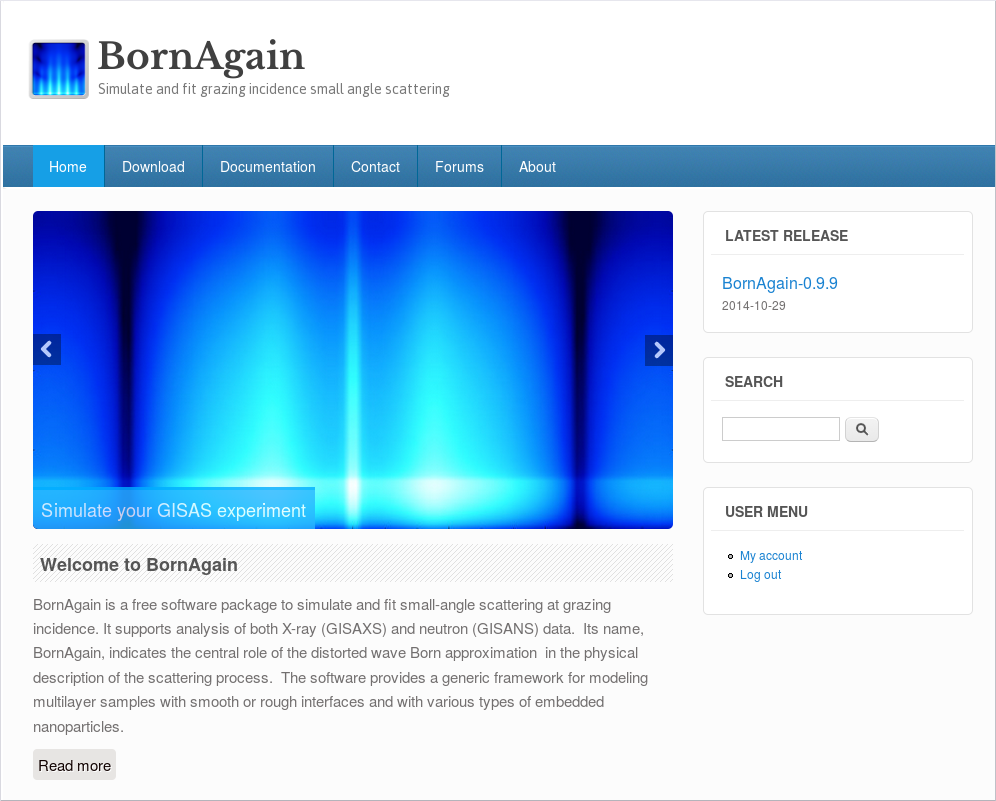
\includegraphics[width=0.99\textwidth]{Figures/website}
\end{center}
\caption{BornAgain project web site.}
\label{fig:nointerf}
\end{figure}


%\section{Quick start on Unix Platforms}
%
%This section shortly describes how to build and install \BornAgain\ 
%from source and run the first simulation on Unix Platforms. 
%Further details about the installation procedure are given in \SecRef{Installation}. \\
%
%\noindent
%{\bf Step I: $~$ installing the third party software}
%\begin{itemize}
%\item compilers: clang  versions $\geq 3.1$ or GCC versions $\geq 4.2$
%\item cmake ($\geq 2.8$)
%\item boost library ($\geq 1.48$)
%\item GNU scientific library ($\geq 1.15$)
%\item fftw3 library ($\geq 3.3.1$)
%\item \Python-2.7, python-devel, python-numpy-devel
%%\item Eigen3 library ($\geq 3.1.0$), optional
%%\item ROOT framework ($\geq 5.34.00$), optional
%\end{itemize}
%\vspace*{2mm}
%
%
%\noindent
%{\bf Step II: $~$ getting the source} \newline
%Download \BornAgain\ source tarball from \url{http://apps.jcns.fz-juelich.de/BornAgain}
%or use the following git repository
%\begin{lstlisting}[language=shell, style=commandline]
%git clone git://apps.jcns.fz-juelich.de/BornAgain.git 
%\end{lstlisting}
%
%\vspace*{3mm}
%
%
%
%\noindent
%{\bf Step III: $~$ building the libraries and executable}
%\begin{lstlisting}[language=shell, style=commandline]
%mkdir <build_dir>; cd <build_dir>;
%cmake -DCMAKE_INSTALL_PREFIX=<install_dir> <source_dir>
%make -j4
%make check
%make install
%\end{lstlisting}
%\vspace*{3mm}
%
%
%\noindent
%{\bf Step IV: $~$ running an example}
%\begin{lstlisting}[language=shell, style=commandline]
%python <install_dir>/share/BornAgain/Examples/python/simulation/ex001_CylindersAndPrisms/CylindersAndPrisms.py
%\end{lstlisting}
%
%
%
%\section{Quick start on Windows Platforms}
%
%\noindent
%{\bf Step I: $~$ installing the third party software} \newline
%The current version of \BornAgain\ requires \Code{Python, numpy, matplotlib} 
%to be installed on the system. If you don't have them already installed,
%you can use \Code{PythonXY} installer available 
%at \url{https://code.google.com/p/pythonxy} which, with default installation options, contains at least these three packages.
%%\BornAgain\ installation.
%\vspace*{2mm}
%
%\noindent
%{\bf Step II: $~$ using BornAgain installation package } \newline
%Windows installation package can be downloaded from \url{http://apps.jcns.fz-juelich.de/BornAgain}.
%Double-click on it to start the installation process. Then follow the instructions.
%\vspace*{2mm}
%
%\noindent
%{\bf Step III: $~$ running the example} \newline
%Run an example located in \BornAgain\ installation directory:
%\begin{lstlisting}[language=shell, style=commandline]
%python C:/BornAgain-<Version>/Examples/python/simulation/ex001_CylindersAndPrisms/CylindersAndPrisms.py
%\end{lstlisting}
%
%
%\section{Getting help}
%Users of the software who encounter problems during the installation
%of the framework or during the run of a simulation can use the web-based issue tracking system
%at
%\url{http://apps.jcns.fz-juelich.de/redmine/projects/bornagain/issues}
%to report a bug. The same system can be used to request new features.
%This system is open for all users in read mode, while 
%submitting bug reports and feature requests are possible only after a simple registration
%procedure.
%
%
%
%
%%Requirements
%
%%Hardware
%%BornAgain is known to work on following platforms:
%%Linux (x86, amd64)
%%MacOS X (x86)
%
%%Software
%%GCC 4.1.2 or above   C/C++ compiler
%%or
%%clang
%%gcc 4.1.2 or above, clang
